\subsection{Duality of Matter}

What led to the development of quantum mechanics was spirited debate about the true nature of light.
Newton was one of the first to throw his hat into the ring; in 1672 he decided to build upon the corpuscular theory coined by Descartes, arguing that light was made up of discrete particles just like everything else.
Problem was, that around the same time Robert Hooke and Christian Huygens performed experiments  that led them to believe light was in fact not a stream of particles but rather a wave.
This wave view of light did a much better job of explaining how light refracted compared to Newtons model.

The position of people beliving that light was in fact a wave, not particles got a lot stronger in 1801 thanks to double slit experiments by Thomas Young.
This was an experiment where there were two slits cut into a screen and light was then shone through it being visible on another screen once it had made it past the slits.
If light was indeed made up of particles, the expectation was that we would see essentially 2 bright spots on the final screenthat corresponded to the two slits.
Instead, what we got was an interference pattern that iss typical of waves.

\begin{figure}[H]
  % https://en.wikipedia.org/wiki/Double-slit_experiment#/media/File:Double-slit.svg
  \centering
  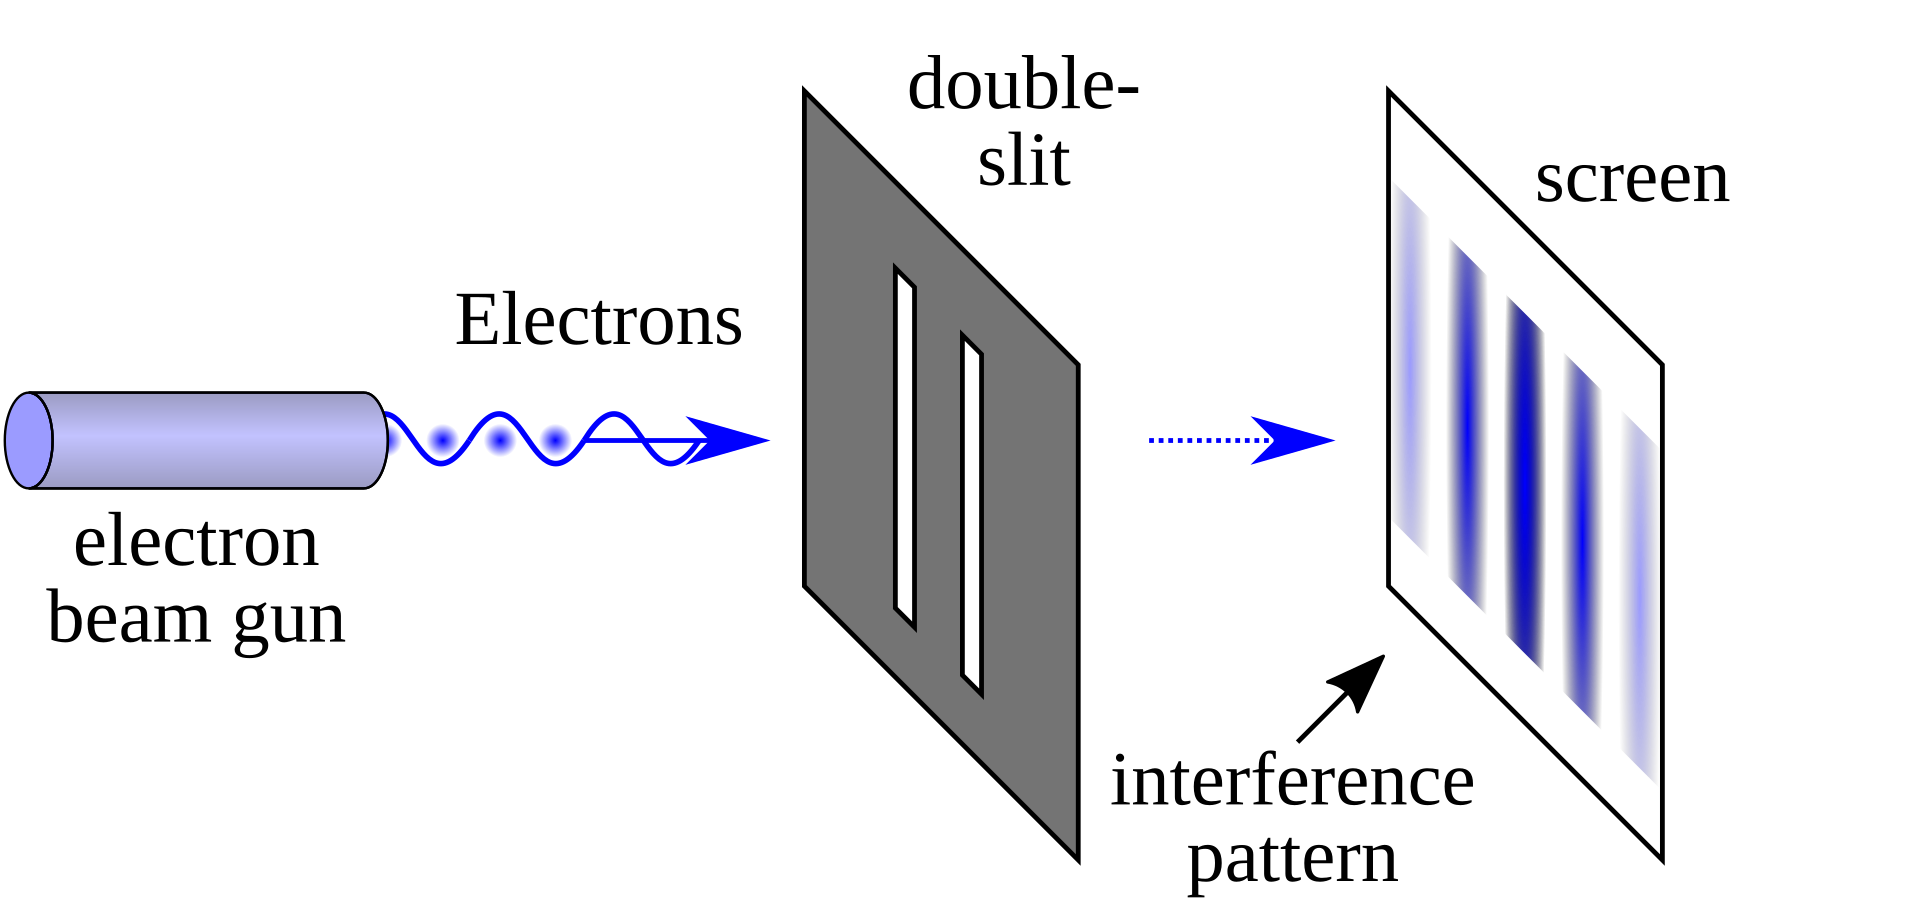
\includegraphics[width=100mm]{figures/doubleSlit.png}
  \caption{Double Slit Experiment}
  \label{doubleSlit}
\end{figure}

At this point, the world is pretty much in the wave camp for the purposes of modelling light, but the idea that light is made of particles was about to be revived from the dead by none other than Max Planck.
